%-- einleitung

\section{Einleitung}

\subsection{Allgemeine Thematik}

In dieser Ausarbeitung werden die wesentlichen Evolutionsstrategien thematisiert.
Dabei handelt es sich um eine Kategorie der evolutionären Algorithmen, die sich seit den 1960er Jahren parallel zu den genetischen Algorithmen entwickelt hat.
Evolutionsstrategien\footnote{\textit{kurz:} ES} stellen wesentliche Modelle der Evolution für Computersimulationen und Anwendungen in der Informatik dar.
Ingo Rechenberg und Hans-Paul Schwefel sind schöpfende Persönlichkeiten, die die Evolutionsstrategien prägten und daraufhin die Rechenberg-Schwefel-Notation zur Modellierung von Evolutionsvorgängen durchsetzten.

\begin{figure}[H]
\centering
\begin{subfigure}[b]{0.45\linewidth}
\centering
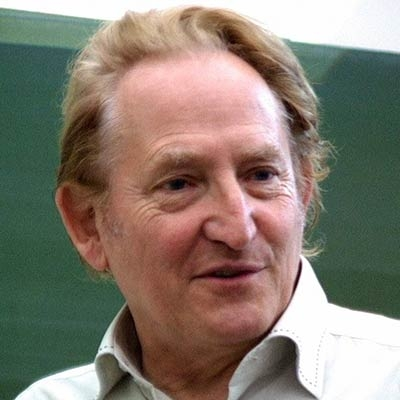
\includegraphics[height=0.6\textwidth]{img/Prof-Dr-Ingo-Rechenberg.jpg}
\caption[Prof. Dr. Ingo Rechenberg]{Prof. Dr. Ingo Rechenberg\protect\footnotemark}
\label{fig:ingorechenberg}
\end{subfigure}
\hfill
\begin{subfigure}[b]{0.45\linewidth}
\centering
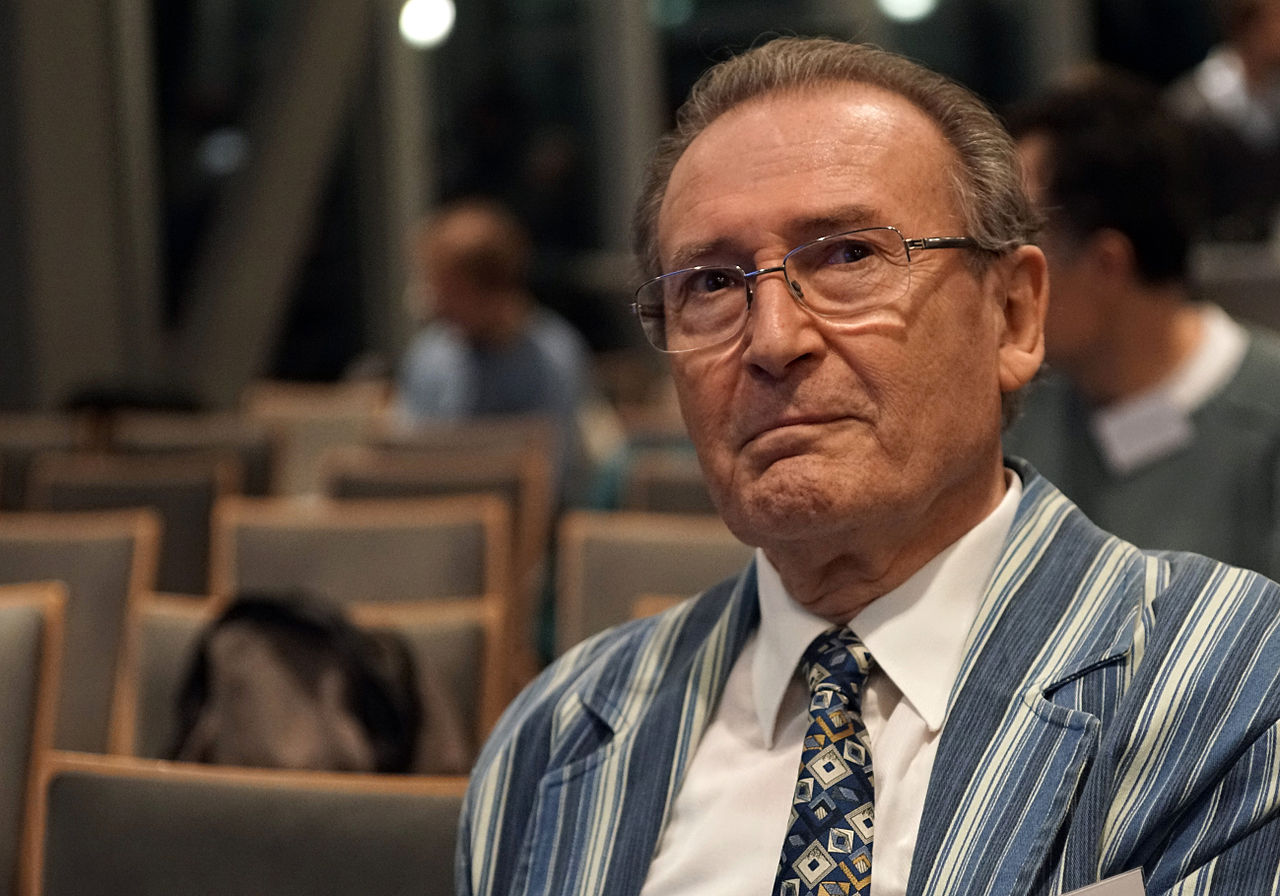
\includegraphics[height=0.6\textwidth]{img/Prof_Dr_Hans-Paul_Schwefel.jpg}
\caption[Prof. Dr. Hans-Paul Schwefel]{Prof. Dr. Hans-Paul Schwefel\protect\footnotemark}
\label{fig:hanspaulschwefel}
\end{subfigure}
\caption{Präger der Evolutionsstrategien}
\label{fig:praeger_der_evolutionsstrategien}
\end{figure}
\footnotetext[4]{\url{https://prominente-redner.de/wp-content/uploads/2019/01/Prof-Dr-Ingo-Rechenberg-als-Redner-buchen-400x400.jpg}}
\footnotetext{\url{https://de.wikipedia.org/wiki/Hans-Paul_Schwefel\#/media/Datei:Prof._Dr._Hans-Paul_Schwefel.jpg}}


Dieses Thema befasst sich mit allgegenwärtigen Optimierungsproblemen, die unter anderem auch technische Anwendung finden.
Bereits 1964 hat Rechenberg an der Universität Berlin mit der einfachsten Form der Evolutionsstrategien eine optimale Einstellung von Gelenkwinkeln einer Gelenkplatte berechnet \cite{schoeneburg}.
Ein weiteres Beispiel für ein kombinatorisches Optimierungsproblem ist das Problem des Handlungsreisenden (\textit{engl.} \enquote{traveling salesman problem}), dessen Bearbeitung im Anschluss an dieser fachlichen Ausarbeitung in einer gesonderten Ausarbeitung im Detail betrachtet wird.

In Abbildung \ref{fig:lokale_globale_maxima} sind die Auswirkungen der Wertfestlegung einzelner Parameter bei einem Optimierungsproblem beispielhaft zu sehen.
Unterschiedliche Kombinationen resultieren in unterschiedlich qualitativen Problemlösungen.
Um gewisse Parametereinstellungen befinden sich lokale Maxima, welche die nächstbeste Lösung im Vergleich zur aktuellen Parameterwahl darstellen. Diese bieten jedoch nur suboptimale Lösungen. Die optimale Lösung wird mit dem finden des globalen Qualitätsmaximum erreicht.

\begin{figure}[H]
\centering
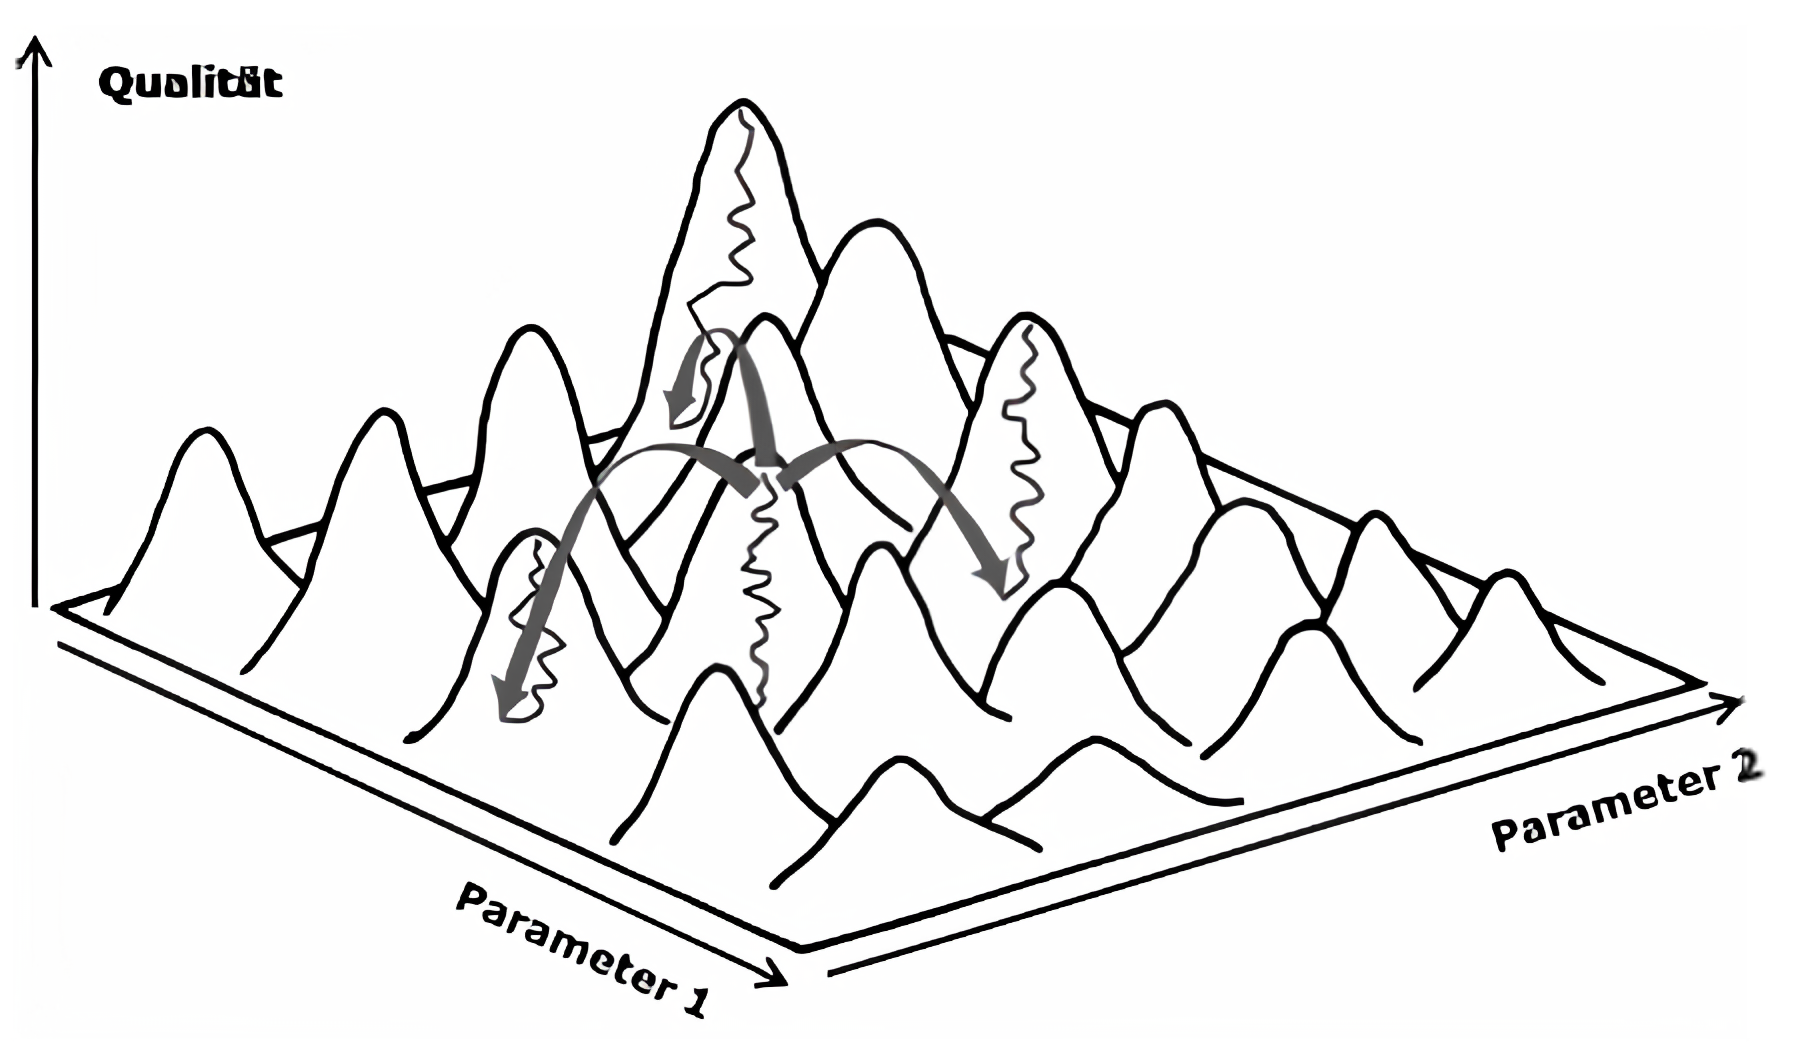
\includegraphics[width=0.65\textwidth]{img/Evolutionsstrategie_lokale_globale_Maxima.png}
\caption[Optimierungsprobleme: lokale Maxima/Minima finden]{Optimierungsprobleme: globales Qualitätsmaximum finden\protect\footnotemark}
\label{fig:lokale_globale_maxima}
\end{figure}
\footnotetext{\url{http://www.bionikvitrine.de/mediapool/99/996537/resources/17835925.png}}

Die Grundidee von evolutionären Algorithmen ist es nun, iterativ eine besser werdende Lösung eines Problems heranwachsen zu lassen.
Die Biologie dient dabei als Ansatzpunkt zur Modellierung einer möglichst stetigen Weiterentwicklung.
Nach dem Grundprinzip \enquote{survival of the fittest} soll sich die Lösung eines Optimierungsproblems über mehrere Generationen hinweg nach und nach in kleinen Anpassungsschritten dem Optimum annähern, bis eine nützliche Konfiguration von Parametern verwendet werden kann.

Abbildung \ref{fig:ablauf_einer_evolution} stellt die allgemeinen Evolutionsschritte sowie deren Ablauf dar.
Algorithmen zur Umsetzung einer speziellen Evolutionsstrategie unterscheiden sich an den Methodiken der Evolutionsschritte (\textit{siehe} Pfeilbeschriftungen).

\begin{figure}[H]
\centering
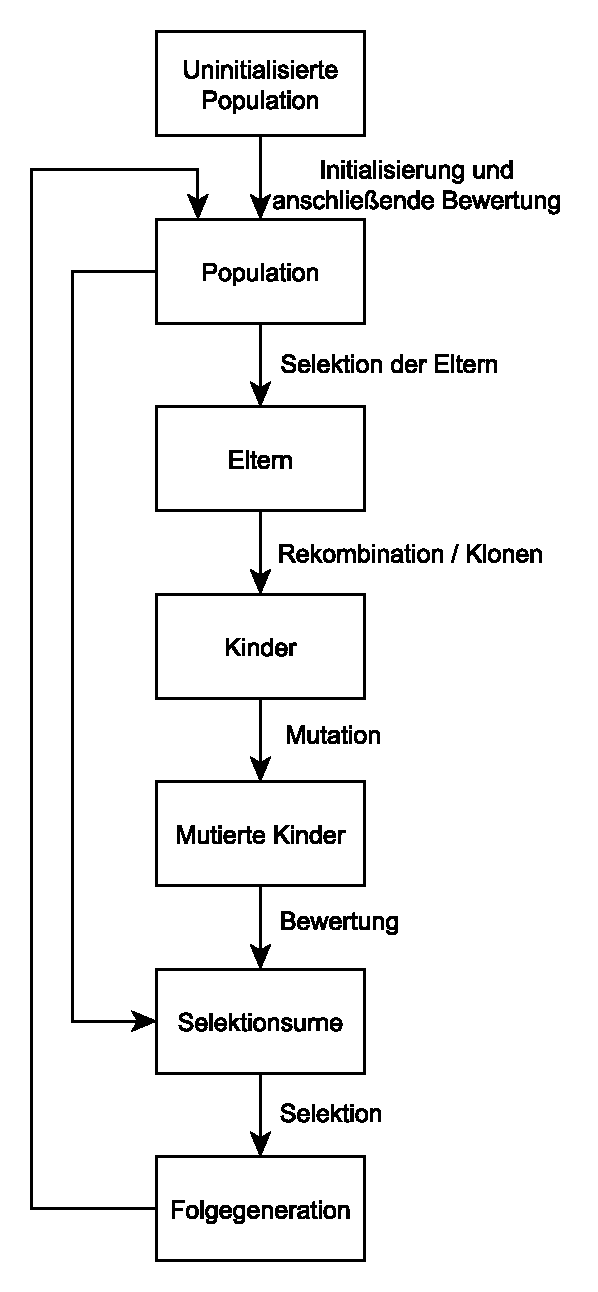
\includegraphics[width=0.4\textwidth]{img/ablauf_einer_evolution.pdf}
\caption[Ablauf einer Evolution]{Ablauf einer Evolution\protect\footnotemark}
\label{fig:ablauf_einer_evolution}
\end{figure}
\footnotetext{\url{http://www.evocomp.de/themen/evolutionsalgorithmen/pic/Evolutionsalgorithmen_Ablauf.gif}}

\pagebreak

Zu Beginn werden Parameterkonfigurationen, sogenannte \enquote{Individuen}, zufällig aufgebaut.
Anschließend werden daraus Eltern nach einem festgelegten Verfahren bestimmt, deren Informationen nach einem Klonvorgang bzw. einer Rekombination mehrerer Eltern an Kinder weitergegeben werden.
Zu einer gewissen Wahrscheinlichkeit werden die nachkommenden Individuen mutiert, bevor sie abschließend anhand einer Qualitätsfunkton nach deren \enquote{Fitness} für die nächste Generation selektiert werden.
Die qualitativ hochwertigsten Nachkommen dienen in der nächsten Iteration als Eltern.
Werden mehrere Individuen über den evolutionären Prozess hinweg beibehalten, spricht man bei einer Sammlung von Individuen von einer \enquote{Population}.

Eine Evolutionsstrategie gewährleistet keinen stetigen Qualitätsfortschritt. Oftmals kann eine Population an einem lokalen Maximum, als an einer suboptimalen Lösung, festhängen. Rückschritte in der Entwicklung sind auch möglich und hängen auch von der gewählten \enquote{Schrittweite} ab. Diese bestimmt, in welchem Maß die Parameterwerte eines von mindestens einem Elter stammenden Nachkommens angepasst werden.

\subsection{Aufbau der Ausarbeitung}

Nachdem die allgemeine Thematik im Grundsatz bekannt ist, wird im nächsten Abschnitt auf die Kodierung der Individuen eingegangen. Anschließend werden grundlegende, unterschiedliche Evolutionsstrategien behandelt, wobei jeweils ein zugehöriger Pseudocode-Abschnitt zur schnellen Umsetzung der jeweiligen Strategie dienen soll.

Dabei werden die Unterschiede zwischen den Evolutionsstrategien angesprochen. Hauptmerkmal der Evolutionsstrategien ist die Evolution. In Hinblick darauf wird die $\frac{1}{5}$-Regel als Grundtechnik und die mutative Schrittweitensteuerung zur Anpassung der Evolution detailliert aufgefasst.

%--